\documentclass[]{beamer}
\mode<presentation>
\usetheme{Frankfurt}
\usepackage{amssymb,amsmath,epsfig,amsthm}
\usepackage{graphicx}
\usepackage{subfloat}
\usepackage{float}
\usepackage[english]{babel}
%\usepackage[latin1]{inputenc}
%\usepackage{times}
\usepackage[T1]{fontenc}
\renewcommand{\baselinestretch}{1.1}
\renewcommand\mathfamilydefault{\rmdefault}
\hypersetup{colorlinks=true,linkcolor=cyan} 

\beamertemplatenavigationsymbolsempty 

%\title{Exploring the Possibility of Floating Orbits for Extreme Mass Ratio Binary Black Holes}
%%\title{Far-field Diffraction of a Vortex Beam}
%\author{Shasvath J. Kapadia}
%\institute{Department of Physics \\ 
\includegraphics[height=0.5cm]{UA_Logo_Horizontal.png}}
%\date{July 30, 2012}
%
\begin{document}
%
%\begin{frame}
%  \titlepage
%
%
%\end{frame}
%slide 1%
\begin{frame}
  \frametitle{Event classification for a gravitational-wave inspiral search \\
 with a sine-Gaussian glitch veto}
\begin{figure}
\vspace*{-0.5cm}
{
  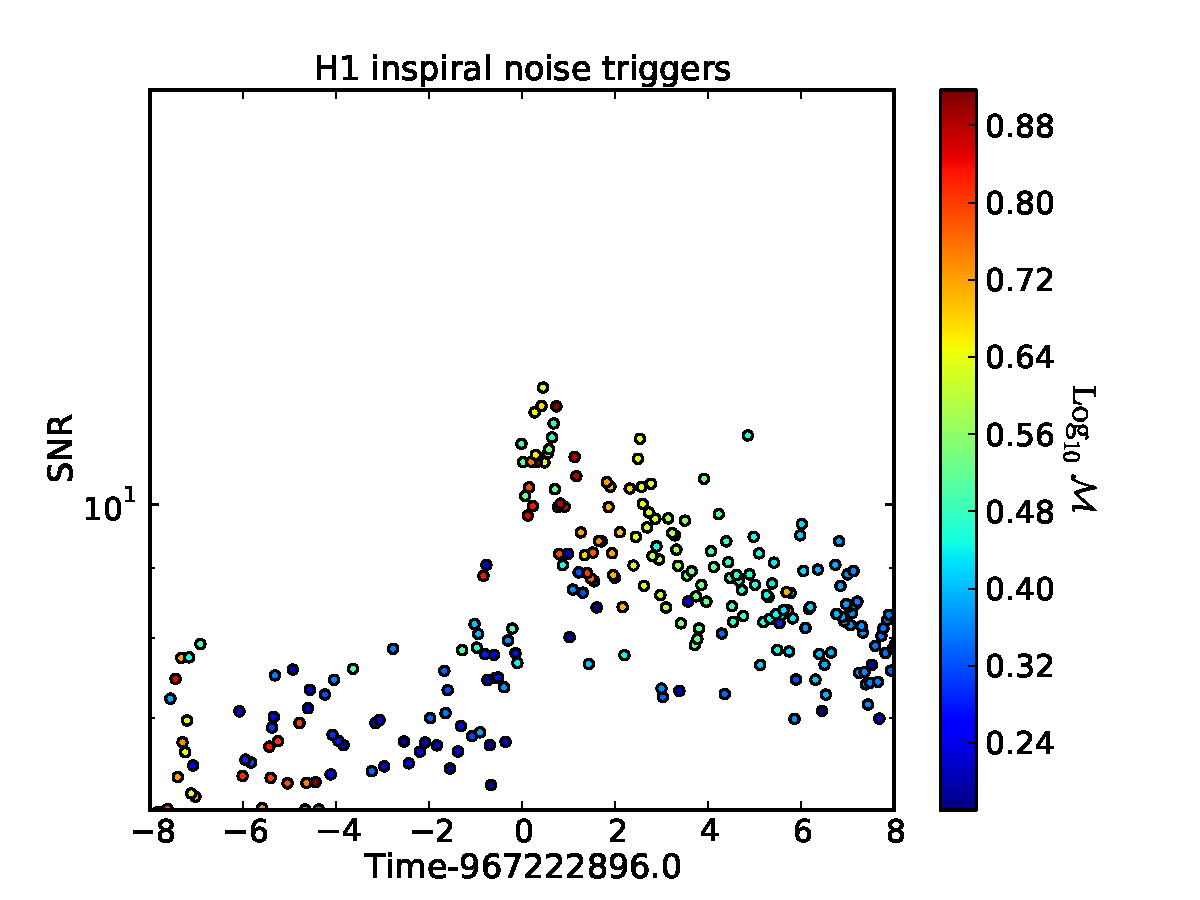
\includegraphics[scale=0.20]{images/H1-inspiral-noise-trigs_POSTER.pdf}
}
\hspace{0cm}
{
  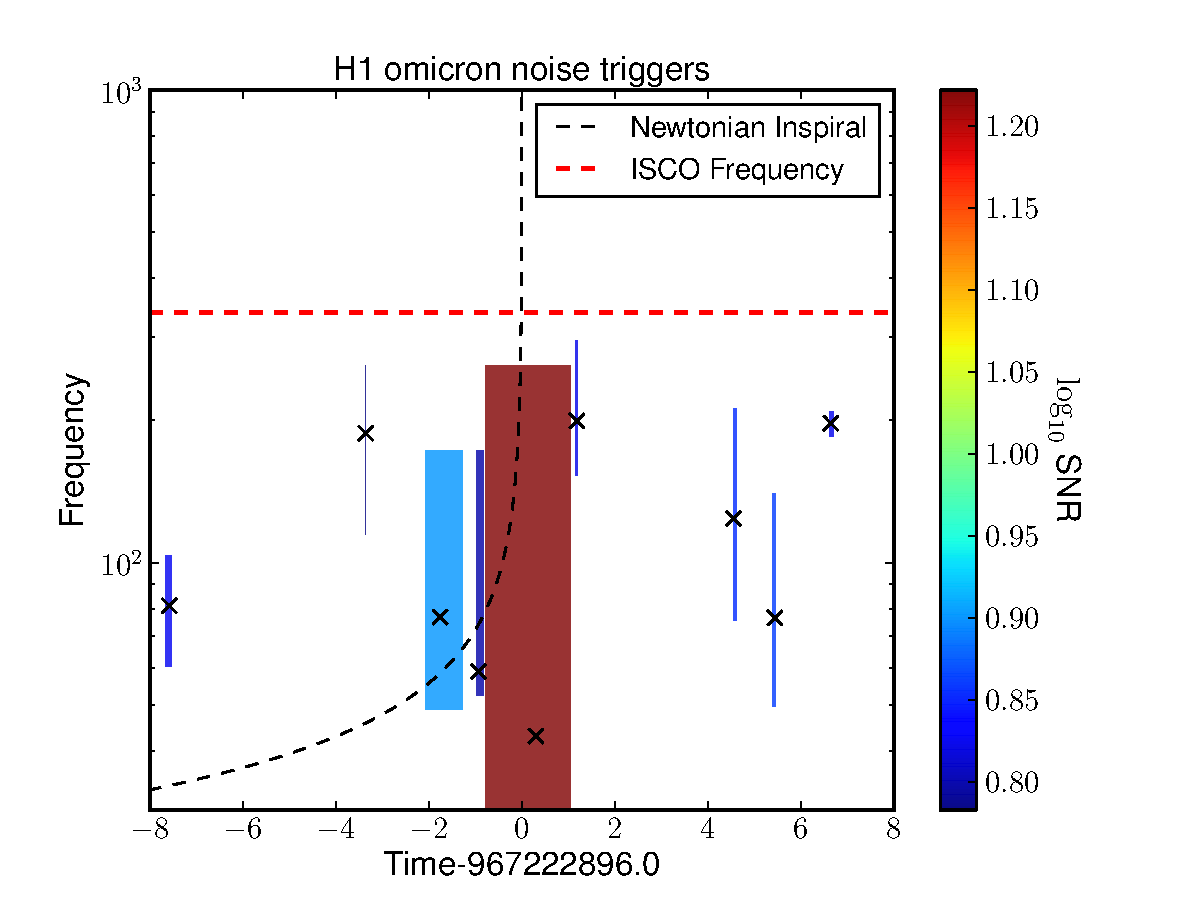
\includegraphics[scale=0.20]{images/H1-omicron-noise-trigs_POSTER.pdf}
}
\vspace*{-0.5cm}
\end{figure}

\begin{itemize}
\item Templated inspiral search in simulated aLIGO data.
\item Separate signal events from high-SNR noise events.
\item Use properties of {\bf multiple} triggers (inspiral + sine-Gaussian). 
\item {\bf Machine learning} multivariate classifier.
\item Improvement in classification w.r.t previous methods.
\end{itemize}
\end{frame}

\end{document}